\documentclass[a4paper,10pt]{article}
\usepackage[utf8]{inputenc}
\usepackage[T1]{fontenc}
% Use correct language package
\usepackage[british]{babel}
\selectlanguage{british}
% Sets page size and margins
\usepackage[top=1.8cm, bottom=1.8cm, left=2cm, right=2cm]{geometry}
% Use multi-line comments
\usepackage{comment}
% math symbols etc.
\usepackage{amsmath}
% making pictures
\usepackage{graphicx}
% making enumerations
\usepackage{enumitem}
% making an appendix
\usepackage{appendix}
% make a wrap figure
\usepackage{wrapfig}
% align caption
\usepackage{caption}

\begin{document}

\section*{Context and theory of this experiment}

\subsection*{Michelson Interferometer}
The Michelson Interferometer uses in it simplest form only 5 optical elements.

\begin{figure}[h]
    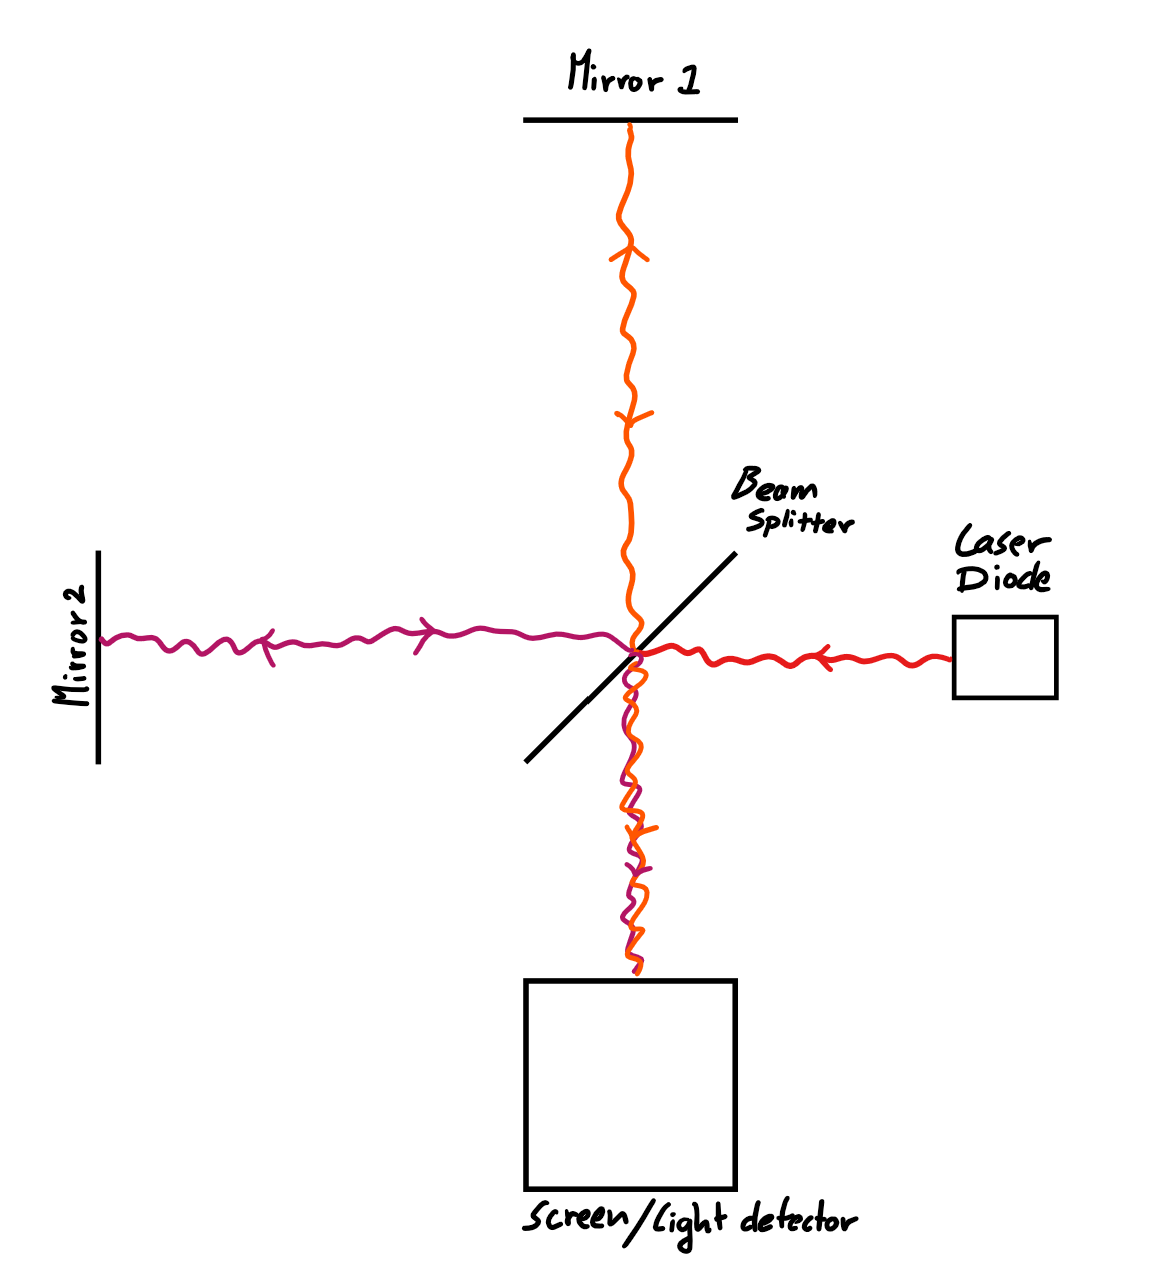
\includegraphics[width=0.49\textwidth]{M_Interferometer.PNG}
    \caption{a) caption.}
    \label{fig:1}
\end{figure}

\end{document}
